\section{Results}
\label{sec:results}

\subsection{Do Augmentation Effects Depend on the Class?}
\label{sec:results_measurement}

Table~\ref{tab:interaction} reports the edit$\times$class interaction test of Section~\ref{sec:measure_tests} for the six dataset--detector pairs, and Fig.~\ref{fig:heatmaps} shows the per-class effect of every edit from which the tests are computed.

\begin{table}[t]
\caption{Edit$\times$Class Interaction Tests in the Edit-Wise Measurement Study (Validation, Three Seeds)}
\label{tab:interaction}
\centering
\footnotesize
\setlength{\tabcolsep}{2.6pt}
\begin{tabular}{@{}llccccl@{}}
\toprule
\textbf{Dataset} & \textbf{Detector} & $|\mathcal{C}|$ & $|\mathcal{O}|$ & $F$ (df) & $p$ & \textbf{Holm} \\
\midrule
RDD2022 & Faster R-CNN & 4 & 12 & 3.73 (33, 88) & $4.5\times10^{-7}$ & -- \\
RDD2022 & RetinaNet & 4 & 12 & 0.79 (33, 88) & 0.77 & -- \\
VOC & Faster R-CNN & 20 & 12 & 1.60 (209, 440) & $2.4\times10^{-5}$ & -- \\
VOC & RetinaNet & 20 & 12 & 1.91 (209, 440) & $1.0\times10^{-8}$ & mosaic \\
dacl10k & Faster R-CNN & 12 & 13 & 2.52 (132, 288) & $4.1\times10^{-11}$ & mosaic, contrast \\
dacl10k & RetinaNet & 12 & 13 & 1.06 (132, 288) & 0.34 & -- \\
\bottomrule
\end{tabular}
\vspace{2pt}

\parbox{\columnwidth}{\footnotesize Holm: edits whose per-edit class contrast remains significant at 5\% after Holm correction across edits.}
\end{table}

\begin{figure*}[t]
\centering
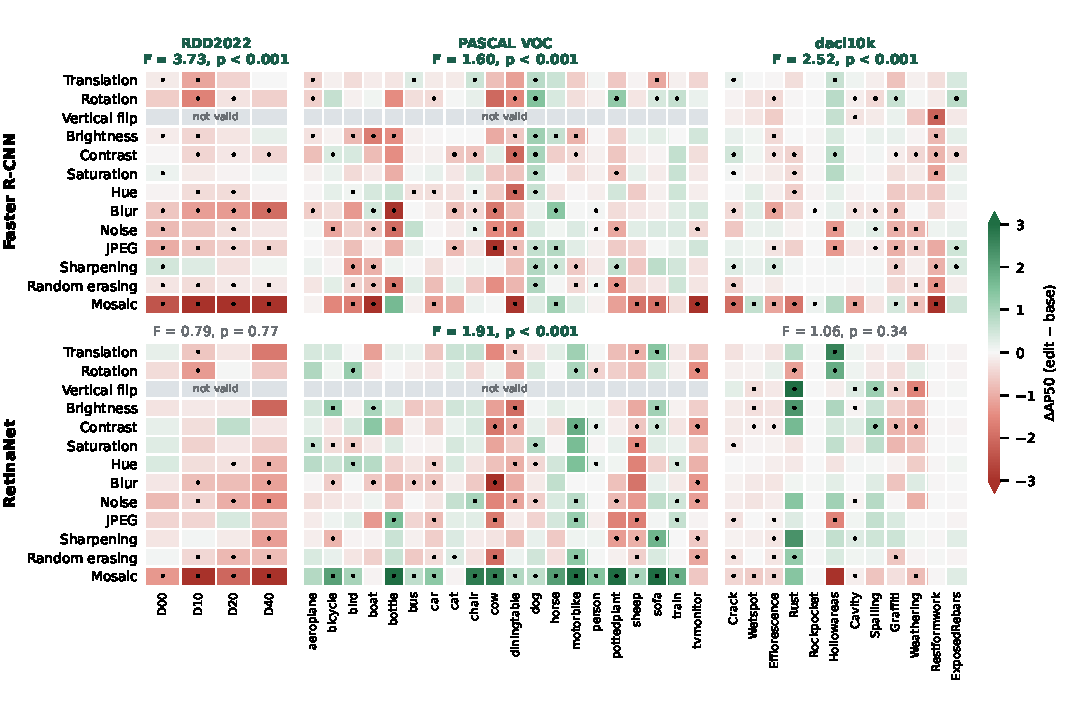
\includegraphics[width=\textwidth]{figures/measurement_heatmaps.pdf}
\caption{Per-class effect of each edit in the edit-wise measurement study (validation, mean over three seeds). Each cell is the change in AP50 when the edit is added to the base recipe; green cells gain and red cells lose. A dot marks a cell whose change has the same sign in all three seeds, which also happens for a quarter of cells without any true effect. Panel titles give the edit$\times$class interaction test of Table~\ref{tab:interaction}, in green when significant at 5\%. Rows whose colour changes sign within a panel are edits whose effect depends on the class; uniformly red rows, such as mosaic on RDD2022, are edits that cost every class.}
\label{fig:heatmaps}
\end{figure*}

\noindent\textbf{The effect of an edit depends on the class.} With Faster R-CNN, the edit$\times$class interaction is significant in all three domains: on RDD2022 ($F(33,88)=3.73$, $p=4.5\times10^{-7}$), on PASCAL VOC ($F(209,440)=1.60$, $p=2.4\times10^{-5}$) and on dacl10k ($F(132,288)=2.52$, $p=4.1\times10^{-11}$). With RetinaNet, it is significant on PASCAL VOC only ($F(209,440)=1.91$, $p=1.0\times10^{-8}$). In four of the six dataset--detector pairs, therefore, how much an edit changes AP50 depends on which class is measured, beyond what the average effect of the edit and the average sensitivity of the class explain.

\noindent\textbf{Two edits carry the dependence that survives correction.} When each edit is tested on its own and the results are corrected across edits, two edits remain significant on dacl10k with Faster R-CNN, mosaic ($p_{\mathrm{Holm}}=0.0003$) and contrast ($p_{\mathrm{Holm}}=0.002$), and one on PASCAL VOC with RetinaNet, mosaic ($p_{\mathrm{Holm}}<0.001$). Contrast on dacl10k is the clearest case of an edit that helps some classes and hurts others: its effect is positive in all three seeds for Crack and Hollowareas, and negative in all three seeds for Efflorescence, Rust, Graffiti, Weathering, Restformwork and ExposedRebars. The classes it hurts include the colour-defined defects named in Section~\ref{sec:intro}, rust and efflorescence, although the study does not test why. Mosaic on PASCAL VOC with RetinaNet is a different case: the classes differ in how much it helps rather than in whether it helps. It raises AP50 by 1.82 on average, its effect is positive in all three seeds for 16 of the 20 classes, and its class means span 7.6 AP50.

\noindent\textbf{Opposite effects on single classes are common but mostly within noise.} Beyond these two edits, several edits have effects of opposite sign on different classes in all three seeds. On dacl10k with Faster R-CNN, mosaic is positive for three classes and negative for six, and sharpening positive for three and negative for two; on PASCAL VOC with Faster R-CNN, rotation is positive for four classes and negative for three, and sharpening and hue are each positive for three and negative for three; on dacl10k with RetinaNet, vertical flip is positive for three and negative for three, although that pair shows no significant interaction. These counts must be read with care. A cell without any true effect has the same sign in all three seeds with probability $1/4$, so with 20 classes about 2.5 such cells per edit and direction are expected from seed noise alone, and the PASCAL VOC counts are of that size. The interaction tests, not these counts, carry the inference.

\begin{table}[t]
\caption{Mean Change in Validation AP50 over Classes for Each Edit (Edit $-$ Base, Three Seeds)}
\label{tab:mean_effects}
\centering
\footnotesize
\setlength{\tabcolsep}{3.2pt}
\begin{tabular}{@{}lrrrrrr@{}}
\toprule
 & \multicolumn{2}{c}{\textbf{RDD2022}} & \multicolumn{2}{c}{\textbf{VOC}} & \multicolumn{2}{c}{\textbf{dacl10k}} \\
\cmidrule(lr){2-3}\cmidrule(lr){4-5}\cmidrule(l){6-7}
\textbf{Edit} & F & R & F & R & F & R \\
\midrule
Mosaic & $-$3.55 & $-$2.93 & $-$0.85 & +1.82 & $-$0.64 & $-$0.51 \\
Blur & $-$1.27 & $-$0.73 & $-$0.34 & $-$0.59 & $-$0.27 & $-$0.02 \\
Rotation & $-$0.75 & $-$0.56 & $-$0.10 & $-$0.06 & +0.05 & +0.03 \\
JPEG & $-$0.67 & $-$0.33 & $-$0.29 & $-$0.19 & $-$0.36 & $-$0.05 \\
Noise & $-$0.52 & $-$0.93 & $-$0.32 & $-$0.21 & $-$0.23 & +0.13 \\
Translation & $-$0.44 & $-$0.63 & $-$0.22 & $-$0.09 & $-$0.03 & +0.18 \\
Contrast & $-$0.29 & +0.08 & $-$0.32 & $-$0.10 & $-$0.12 & +0.07 \\
Random erasing & $-$0.25 & $-$0.51 & $-$0.37 & $-$0.12 & $-$0.24 & +0.04 \\
Hue & $-$0.21 & $-$0.31 & $-$0.10 & $-$0.04 & $-$0.16 & $-$0.10 \\
Brightness & $-$0.17 & $-$0.70 & $-$0.26 & $-$0.05 & $-$0.01 & +0.13 \\
Saturation & $-$0.01 & $-$0.24 & $-$0.13 & $-$0.03 & $-$0.10 & $-$0.08 \\
Sharpening & +0.14 & $-$0.39 & $-$0.08 & $-$0.17 & $-$0.01 & +0.35 \\
Vertical flip & -- & -- & -- & -- & $-$0.31 & +0.19 \\
\bottomrule
\end{tabular}
\vspace{2pt}

\parbox{\columnwidth}{\footnotesize F: Faster R-CNN; R: RetinaNet. --: edit not valid for the dataset.}
\end{table}

\noindent\textbf{Most edits cost a little in the short run, and mosaic stands out.} Averaged over classes, most edits lower validation AP50 slightly in the three-epoch continuation, and no edit raises AP50 consistently for all classes of a dataset (Table~\ref{tab:mean_effects}). Mosaic is the exception in both directions. It is strongly negative on RDD2022 ($-3.55$ AP50 with Faster R-CNN and $-2.93$ with RetinaNet), mildly negative on dacl10k ($-0.64$ and $-0.51$) and negative on PASCAL VOC with Faster R-CNN ($-0.85$), but positive on PASCAL VOC with RetinaNet ($+1.82$). Because the continuation lasts only three epochs, these averages describe the early effect of an edit; the next paragraph examines how far they carry over to full training.

\noindent\textbf{Short runs agree moderately with full training.} For RDD2022 with Faster R-CNN, the base recipe and four edits retrained with the full 20-epoch schedule give a Spearman correlation of $\rho=0.56$ between short-run and full-run per-class effects over 16 edit--class cells, with a 95\% bootstrap interval of $[0.04,\,0.86]$. The correlation passes the threshold of 0.5 set before the run, but the interval is wide. We therefore treat the signs of the short-run effects as moderately reliable and their sizes as indicative only.

\noindent\textbf{RetinaNet shows no class dependence on RDD2022 and dacl10k.} For these two pairs the interaction is not significant ($F=0.79$, $p=0.77$ and $F=1.06$, $p=0.34$), and the differences between classes are of the size expected from seed-to-seed variation. We report this as found. One possibility, which this study does not test, is that three epochs are too few for class differences to appear in RetinaNet's dense head; the agreement check above covers Faster R-CNN only.

Together, these results support the premise of CUA for Faster R-CNN in all three domains and for RetinaNet on PASCAL VOC. For RetinaNet on RDD2022 and dacl10k they do not, and in those two settings CUA is expected to perform like shared-utility augmentation.

\subsection{Does CUA Exploit Class Dependence?}
\label{sec:results_comparison}

\todo{Section VI.B is written when the policy comparison finishes: main comparison (Table~\ref{tab:main}), differences with intervals (Fig.~\ref{fig:forest}), estimator agreement (Fig.~\ref{fig:agreement}), ablations (Table~\ref{tab:ablations}), and secondary metrics: AP50:95, AP by object size, false-positive images on damage-free RDD2022 images, and estimator overhead on every dataset and detector.}

\begin{table*}[t]
\caption{Test Macro AP50 of the Compared Policies (Mean $\pm$ s.d.\ over Three Seeds)}
\label{tab:main}
\centering
\footnotesize
\todo{Insert main\_table.tex: Base, Uniform, Measured-effect, Shared-utility and CUA for each of the six dataset--detector pairs.}
\end{table*}

\begin{figure}[t]
\centering
\begin{tikzpicture}
  \node[draw=cuaText, dashed, rounded corners=5pt, fill=cuaGrey!45, minimum width=0.97\columnwidth, minimum height=4cm, text width=0.8\columnwidth, align=center, font=\sffamily\footnotesize] {\todo{Forest plot: CUA $-$ shared-utility and CUA $-$ best simple baseline for each dataset--detector pair. Thin line: seed $t$ interval; thick line: image bootstrap.}};
\end{tikzpicture}
\caption{\todo{Caption written with the results.}}
\label{fig:forest}
\end{figure}

\begin{figure}[t]
\centering
\begin{tikzpicture}
  \node[draw=cuaText, dashed, rounded corners=5pt, fill=cuaGrey!45, minimum width=0.97\columnwidth, minimum height=4cm, text width=0.8\columnwidth, align=center, font=\sffamily\footnotesize] {\todo{Estimator agreement: mean estimated class utility against measured $\bar\Delta(o,c)$, one point per edit--class cell, with Spearman $\rho$ and its interval.}};
\end{tikzpicture}
\caption{\todo{Caption written with the results.}}
\label{fig:agreement}
\end{figure}

\begin{table}[t]
\caption{Ablations of CUA on Validation (Faster R-CNN, Three Seeds)}
\label{tab:ablations}
\centering
\footnotesize
\todo{No harm block; no identity candidate; inverse-AP class weights; on RDD2022 and dacl10k.}
\end{table}

\section{Discussion and Limitations}
\label{sec:discussion}

\todo{Discussion, written with the policy comparison: when class information helps, and what it costs.}

\noindent\textbf{Limitations.} The per-class effects were measured in short continuations, and their agreement with full training was checked on one dataset and one detector only, with a wide interval. We did not run a class-targeted study that applies an edit only inside the boxes of one class, so the measured effects combine the direct effect of an edit on a class with its effect through the other objects and the background. We also did not compare CUA with a tolerance-gated controller, so the advantage of a benefit signal over a recognition signal is argued in Section~\ref{sec:related} rather than measured. Each edit has a single strength, the labels are boxes rather than masks, copy-paste augmentation is not covered, and the evaluation spans three domains. Finally, CUA is evaluated with Faster R-CNN and RetinaNet only; extending it to real-time detectors such as YOLO~\cite{bochkovskiy2020yolov4} is left to future work.

